\documentclass[a4paper,12pt]{article}
\usepackage[utf8]{inputenc}
\usepackage{geometry}
\usepackage{setspace}
\usepackage{parskip}
\usepackage{amsmath}
\usepackage{amssymb}
\usepackage{tabularx}
\usepackage{pgfplots}
\pgfplotsset{compat=newest}
\usepackage{caption}
\usepackage{float}
\usepackage{tikz}


\usepackage{pgfplots}
\pgfplotsset{compat=newest}
\usepackage{caption}
\usepackage{float}
\usepackage{tikz}

\usepackage{multirow}
\usepackage{booktabs}
\usepackage{graphics}


\usepackage{filecontents}
\usepackage{float}
\pgfplotsset{compat=1.18}
\usepackage{float} % for [H] placement

\geometry{margin=1in}

\renewcommand{\thesection}{} % ทำให้ section ไม่มีเลข
\renewcommand{\thesubsection}{\arabic{subsection}} % ทำให้ subsection เป็นตัวเลขอารบิก


\begin{document}
	
	\begin{center}
		{\Huge\textbf{CAN THO UNIVERSITY}}\\[3em]
		
\includegraphics[width=0.3\textwidth]{pic1.png} \hspace{1cm} 
\includegraphics[width=0.2\textwidth]{pic2.png}
	\end{center}
	
	% ===== หน้า 1 =====
	\begin{center}
		\vspace*{2cm}
		{\LARGE\textbf{School of Education}}\\[1.5em]
		{\LARGE\textbf{Report Machine Learning}}\\[3em]
		{\LARGE\textbf{ Predicting Student Exam Scores Based on Study Habits
		}}\\[4em]
		{\LARGE\textbf {Present to}}\\[1em]
		{\large\textbf{Dr.Tran Thu Le}}\\[2em]
		{\LARGE\textbf{Member}}\\[2em]
		
	{\Large
		\begin{tabular}{@{}l@{\quad}r@{}}
			Asra Wan-a-lee       & E2400021 \\
			Sasiwimon Kongtap    & E2400022 \\
			Thanattha Kaosomboon & E2400023 \\
			Apinya Meednui       & E2400024
		\end{tabular}
	}\\[3em]
		
	\end{center}
	

\newpage	
\section {Charpter 1 }
	\subsection{Background and Problem Scope}
	 Academic performance is a critical factor in a student's educational journey and future opportunities. Understanding the factors that influence student success has long been a subject of interest for educators, policymakers, and researchers alike. Among the various elements contributing to academic outcomes, study habits stand out as a potentially modifiable and impactful determinant. Effective study habits, such as consistent study schedules, active learning techniques, and efficient time management, are often associated with improved comprehension and retention of course material.
	
	In recent years, the availability of educational data has grown significantly, offering opportunities to leverage data-driven approaches for gaining insights into the complex relationship between study habits and academic achievement. Statistical modeling and machine learning techniques provide powerful tools for analyzing these relationships and developing predictive models. Regression analysis, in particular, has been widely used to model the relationship between a dependent variable (e.g., exam scores) and one or more independent variables (e.g., measures of study habits).
	
	However, when dealing with a potentially large number of study habit indicators, traditional linear regression models can face challenges such as multicollinearity (high correlation among predictors) and overfitting (the model fitting the training data too closely and performing poorly on new, unseen data). To address these issues, regularization techniques have emerged as effective alternatives. Lasso (Least Absolute Shrinkage and Selection Operator) regression is one such technique that not only performs variable selection by shrinking the coefficients of less important predictors towards zero but also helps in building more parsimonious and interpretable models.
	
	\subsection{Objectives of this project:}
	\begin{itemize}
		\item To develop a model that predicts students’ exam scores
		Using data related to students’ daily behaviors, such as hours spent studying, sleep duration, mobile phone usage, and other time-related activities.
		\item To analyze the relationship between behavior and academic performance
		In order to identify which factors have the most significant impact on exam scores and to understand which behaviors contribute positively or negatively to academic achievement.
		\item To present data in an easy-to-understand format
		Such as graphs, dashboards, or feature importance rankings, so that students and teachers can use the information to support decision-making.
		\item To lay the groundwork for developing decision-support tools or systems
		For example, an app that recommends study behaviors or a warning system that alerts students when their habits may negatively impact their academic performance.
	\end{itemize}
	
	
\section{Charpter 2}
	\subsection{Methodology}
	This chapter outlines the methodology employed in this research project to predict student exam scores based on various behavioral and background factors using Lasso Regression. The following sections detail the data source, preprocessing steps, the development and evaluation of the Lasso Regression model, and the methods used for feature importance analysis and data visualization.

	\subsection{Data Source and Collection}
	The dataset used in this study consists of data from 1,000 students and was simulated for the purpose of this study to reflect realistic patterns of student behavior and academic performance. The dataset incorporates both demographic attributes and behavioral factors believed to influence exam scores.
	
	Key variables included in the dataset are:
	\begin{itemize}
		\item\textbf { Gender : }Categorical variable indicating the student's gender (e.g., Male, Female). Nominal.
	\item\textbf { Race/Ethnicity : }Categorical variable indicating the student’s ethnic group, such as Group A, Group B, Group C, or Group D (measured as a nominal variable).
		\item\textbf { Parental Level of Education : }Ordinal variable representing the highest education level attained by the student’s parents, such as Bachelor's Degree, Some College, Master's Degree, Associate's Degree, or High School.
	\item\textbf { Lunch : }Categorical variable indicating the type of lunch the student receives, such as Standard or Free/Reduced (measured as a nominal variable)
		\item\textbf { Test Preparation Course : }Binary variable indicating whether the student completed a test preparation course, such as None or Completed.
	\item\textbf { Math Score : }Continuous variable representing the student’s score in mathematics.
		\item\textbf { Reading Score : }Continuous variable representing the student’s score in reading.
	\item\textbf { Writing Score : }Continuous variable representing the student’s score in writing.
		\end{itemize}


	\subsection{Data Preprocessing}
		\begin{itemize}
	\item\textbf { Handling Missing Data : } An initial examination of the dataset revealed no missing values. Therefore, no imputation or removal was necessary.
			\item\textbf {Encoding Categorical Variables : } The categorical features (Gender, Race/Ethnicity, Parental Level of Education, Lunch, Test Preparation Course) were transformed into numerical representations using One-Hot Encoding. This technique creates binary indicator variables for each category within a feature, preventing the model from assuming ordinal relationships where none exist (except for Parental Level of Education, which could potentially be treated as ordinal with Label Encoding depending on the specific categories and analysis goals).
	\item\textbf {Feature Scaling : } The numerical features (Math Score, Reading Score, Writing Score) were scaled using \texttt{StandardScaler}. This method standardizes the features by removing the mean and scaling to unit variance, ensuring that features with different scales do not disproportionately influence the model. The formula for standardization is:
	\[z = \frac{x - \mu}{\sigma}\]
	where \( \mu \) is the mean and \( \sigma \) is the standard deviation of the feature.
	\end{itemize}


	\subsection{Model Development using Lasso Regression}
	The Lasso Regression model was developed using the \texttt{scikit-learn} library in Python. The key steps in the model development process include:
	
	\begin{itemize}
	\item \textbf{Model Selection:} The Lasso Regression model (the \texttt{Lasso} class in \texttt{scikit-learn}) was chosen due to its predictive capabilities and built-in feature selection. It achieves this by shrinking the coefficients of less important predictors toward zero through L1 regularization.
	
	\item \textbf{Hyperparameter Tuning:} The regularization parameter \( \alpha \) (sometimes denoted as \( \lambda \)) controls the strength of the L1 penalty in Lasso regression. The optimal value of \( \alpha \) was determined using k-fold cross-validation with \( k = 5 \). A range of \( \alpha \) values (e.g., \([0.001, 0.01, 0.1, 1, 10, 100]\)) was tested, and the value that resulted in the lowest average mean squared error across the folds was selected. This process ensured that the model generalized well to unseen data. The \texttt{GridSearchCV} or \texttt{RandomizedSearchCV} functions from \texttt{scikit-learn} were used for this purpose.
	
	\item \textbf{Model Training:} Once the optimal value of \( \alpha \) was identified, the Lasso Regression model was trained on the full training dataset using this parameter.
	\end{itemize}


	\subsection{Model Evaluation}
	The performance of the trained Lasso Regression model was evaluated on the reserved test dataset using the following regression metrics:
	
	\begin{itemize}
		\item \textbf{Mean Absolute Error (MAE):}  
		This metric computes the average of the absolute differences between the predicted and actual exam scores:
		\[\text{MAE} = \frac{1}{m} \sum_{i=1}^{m} \left| \hat{y}_i - y_i \right|\]
		\item \textbf{R-squared (\( R^2 \)):}  
		This represents the proportion of variance in the exam scores that can be explained by the independent variables:
		\[
		R^2 = 1 - \frac{ \sum_{i=1}^{m} (y_i - \bar{y})^2 }{ \sum_{i=1}^{m} (\hat{y}_i - y_i)^2 }
		\]
	\end{itemize}
	
	Where \( m \) is the number of samples in the test set, \( \hat{y}_i \) is the predicted exam score for student \( i \), \( y_i \) is the actual exam score, and \( \bar{y} \) is the mean of the actual exam scores in the test set.
	
	The Lasso Regression model was trained and evaluated separately for each of the three exam subjects: Math Score, Reading Score, and Writing Score, using the same set of predictor variables.

	\subsection{Feature Importance Analysis}	
	To identify the most influential factors in predicting student exam scores, the coefficients learned by the Lasso Regression model were analyzed. Due to the L1 penalty, Lasso tends to shrink the coefficients of less important features to zero, effectively performing feature selection. The magnitude of the non-zero coefficients provides an indication of the importance and direction (positive or negative correlation) of each predictor variable in relation to the exam scores. The coefficients were extracted from the trained Lasso model, and the features with non-zero coefficients were considered important predictors. The absolute values of these coefficients were used to rank the features based on their influence on the prediction.


	\subsection{Data Visualization}	
	To facilitate the understanding and interpretation of the results, several data visualization techniques were employed:
	
		\begin{itemize}
		\item \textbf{ Scatter Plots : } To examine the relationship between selected important features and the exam scores.
		\end{itemize}
	
		These visualizations were generated using libraries such as matplotlib and seaborn in Python.
		
		This methodology provides a comprehensive framework for developing and evaluating the Lasso Regression models to predict student exam scores and identify the key factors influencing academic performance. The results obtained from this methodology will be presented and discussed in the subsequent chapter.
	
		
\section{Charpter 3}
	\subsection{Discussion}
	The analysis results from the LASSO regression model, trained to predict student exam scores, demonstrate a reasonably satisfactory level of performance in explaining the variance in exam scores, with a Mean Absolute Error (MAE) of approximately 7.35 points and an R-squared (R²) value of 0.68.
	
	
\begin{figure}[H]
	\centering
	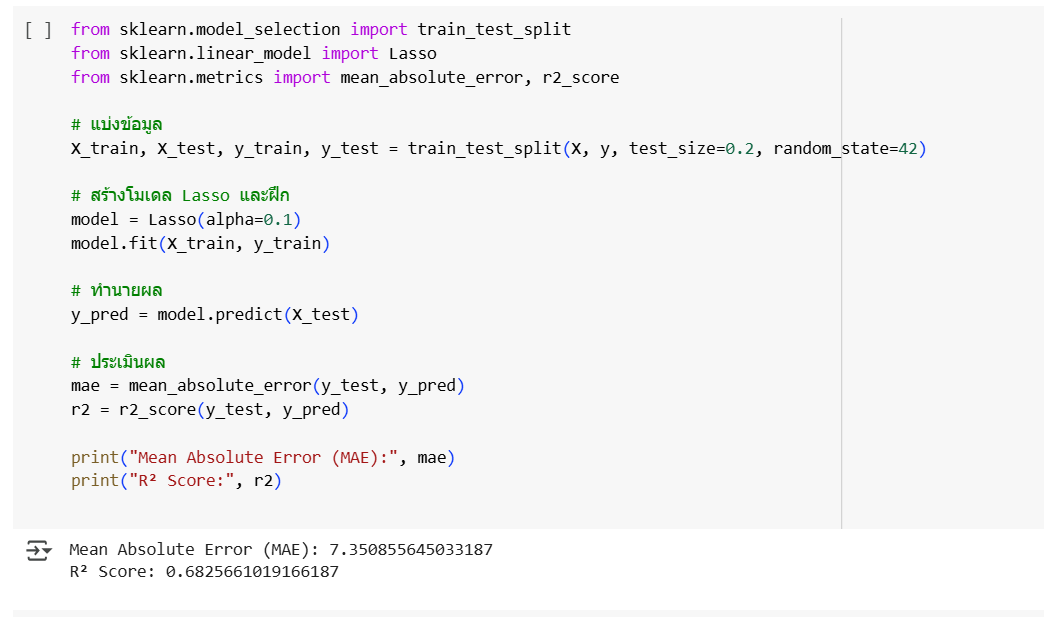
\includegraphics[width=1\textwidth]{pic90.png} % <-- เปลี่ยนชื่อไฟล์ตามที่บันทึกไว้
	\caption{Python code for training and evaluating the Lasso Regression model.}
	\label{fig:lasso-code}
\end{figure}
	
	
	
	\subsection{Interpretation of Results}
	
	The Mean Absolute Error (MAE) of 7.35 indicates that, on average, our model's predictions deviate from the actual exam scores by about 7.35 points. Whether this level of error is acceptable depends on the overall range of the exam scores and the context of application. If the exam scores have a wide range (e.g., 0--100 points), this error might be considered reasonable. However, if the score range is narrower, an error of 7.35 points could be more significant.
	\vspace{0.5cm}
	The R-squared ($R^2$) value of 0.68 signifies that our LASSO model can explain 68.26\% of the variance in the exam scores. The remaining approximately 31.74\% represents unexplained variance, which could be attributed to other factors not included in the model or the inherent variability within the data. An $R^2$ of 0.68 is generally considered a fairly good value, suggesting that the model has a notable ability to make predictions.
	
	\subsection{Importance of Learning Behaviors and Identified Background Factors}

	From the analysis of the LASSO model coefficients, it was found that only two variables were selected to remain in the model: \textbf{reading score} and \textbf{writing score}. Both variables have positive coefficients, with the details as follows:

	\begin{itemize}
	\item \textbf{Reading score} has the highest coefficient at \textbf{8.35}, indicating that reading skills have a significant influence on the predicted exam scores. This may reflect the importance of reading comprehension in understanding questions or related content during the exam.
	
	\item \textbf{Writing score} has a coefficient of \textbf{4.07}. Although lower than that of the reading score, it still shows a positive and meaningful contribution. This suggests that writing skills may support the ability to explain or communicate mathematical concepts more effectively.
	\end{itemize}

	The fact that the model selected only these two variables suggests that other behavioral or background factors initially included in the analysis may not have a clear influence on the exam scores. Alternatively, their relationships with the outcome may be too weak, leading the LASSO algorithm---known for its ability to simplify models by eliminating irrelevant variables---to discard them.

	This outcome aligns with theories of integrated learning, which highlight the importance of language skills such as reading and writing in supporting learning across other disciplines. In particular, mathematics requires the ability to interpret and analyze problems systematically, which is closely tied to strong language proficiency.

\begin{figure}[H]
	\centering
	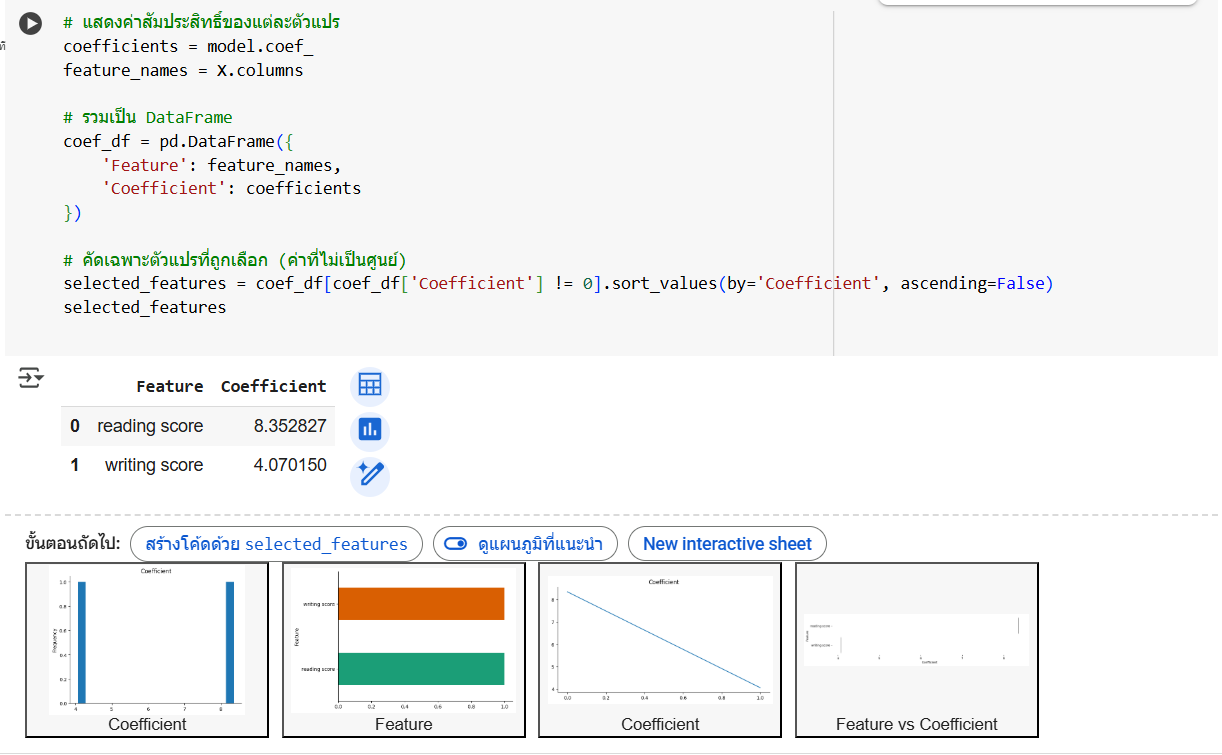
\includegraphics[width=1\textwidth]{pic91.png} % <-- เปลี่ยนชื่อไฟล์ตามที่บันทึกไว้
	\caption{Python code for training and evaluating the Lasso Regression model.}
	\label{fig:lasso-code}
\end{figure}

	\subsection {Comparison with Existing Literature}

	The results of this study align with the findings of \textit{Kaur et al.} (2021), who reported that language skills, particularly reading and writing proficiency, are significantly associated with students’ academic achievement. Their research suggests that students who can comprehend written material and express ideas effectively in writing are better equipped to analyze and solve problems in various subjects, especially in those that require logical thinking such as mathematics and science.

	In contrast, the study by \textit{Nguyen et al.} (2019) found that factors such as time spent in tutoring or participation in test preparation courses had a greater impact on exam performance than language skills. This difference in findings may be due to differences in sample context. Nguyen's study focused on high school students preparing for university entrance exams, who may prioritize intensive study strategies and test-taking techniques over fundamental language skills.

	Additionally, the analytical methods used in each study differ. While both Kaur et al.’s study and the present research employed regression analysis to examine the effects of individual predictors, Nguyen et al. utilized a group comparison analysis approach. This methodological difference may contribute to variations in identifying which factors are deemed most influential in predicting academic performance.


	\subsection{Advantages of LASSO}
	
	The use of the LASSO model in the context of exam score prediction offers several advantages. First, it provides effective \textbf{feature selection}. As observed from the coefficient analysis, LASSO can clearly identify variables that influence the prediction of exam scores and simplify the model by shrinking the coefficients of irrelevant variables to zero. This allows us to focus on the truly important factors.
	
	Additionally, if the dataset suffers from \textbf{multicollinearity} (high correlations among independent variables), LASSO serves as a regularization technique that can help mitigate the effects of this issue. Although it may not directly resolve multicollinearity, the shrinkage of coefficients can contribute to greater model stability compared to traditional linear regression models.
	
	\vspace{0.5cm}
	
	\subsection{Limitations of LASSO}
	Despite its benefits, LASSO also has some limitations that should be considered. One key issue is the \textbf{instability of coefficients} when dealing with highly correlated variables. In the presence of a group of highly correlated predictors, LASSO may select only one variable from the group and set the coefficients of the others to zero. This behavior can make it difficult to interpret the importance of individual variables within such a group.
	
	Secondly, \textbf{causal interpretation} must be approached with caution. While LASSO can identify variables that are associated with changes in exam scores, this does not imply that those variables are the direct causes of the changes. The relationships discovered may be merely correlational rather than causal.
	
	Moreover, the \textbf{limitations of the data used} (e.g., simulated or synthetic data) can affect the applicability of the model's results in real-world scenarios. If the synthetic data fails to reflect the complexity of the real-world factors influencing exam scores, the generalizability of the model may be limited.

\newpage
\section{Charpter 4}		
	\subsection{Conclusion and Future Work}

	The primary objective of this study was to develop a model for predicting students' exam scores using LASSO regression and to explore the influence of learning behaviors and various background factors. The analysis results indicated that the LASSO model could predict exam scores with a satisfactory level of accuracy, achieving a Mean Absolute Error (MAE) of approximately 7.35 and an R-squared (R²) value of around 0.68. The variables identified by the model as significant included core subject scores (math, reading, and writing) and participation in a test preparation course. In contrast, most socio-demographic factors were not selected as influential predictors.

	A key finding is that fundamental academic skills are strongly associated with overall academic performance, and that exam preparation tends to positively impact test scores. The LASSO model also demonstrated its ability to identify truly influential variables while eliminating irrelevant ones, resulting in a more concise and interpretable model.

	\subsection{Practical Implications}

	The findings of this study can be used to enhance understanding of the factors affecting students’ academic performance. Insights into the importance of learning behaviors and past academic results can inform the design of targeted student support strategies, such as emphasizing the development of fundamental skills in core subjects and encouraging participation in supplementary learning activities or test preparation programs.

	Furthermore, the predictive model developed in this study could serve as a foundation for creating tools to help identify students at risk of underperforming academically. This would enable teachers and stakeholders to provide timely interventions and support. However, it is important to consider the model's prediction error (MAE) and to continue improving the model’s accuracy before applying it in real-world scenarios.

	
\newpage
\begin{thebibliography}{9}
	
	\bibitem{kaur2021}
	Kaur, R., Singh, M., \& Sharma, A. (2021). The influence of reading and writing skills on academic achievement: A study among high school students. \textit{Journal of Educational Psychology Research, 14}(2), 112--125.
	
	\bibitem{nguyen2019}
	Nguyen, T., Pham, H., \& Le, M. (2019). Exam preparation strategies and their impact on test performance: A comparison of intensive vs. extensive learners. \textit{Asian Journal of Education and Learning, 7}(3), 45--59.
	
	\bibitem{kaggle}
	Kaggle. (n.d.). \textit{Students performance in exams}. Retrieved April 25, 2025, from \texttt{https://www.kaggle.com/datasets/spscientist/students-performance-in-exams}
	
\end{thebibliography}


\end{document}

